\chapter{Solution Model}
\label{ch:Model}

Design decisions, its rationale and implemetation notes. this in ther and that in there

\section{Operationalization}
We document here how we tranform/reduce the breast cancer detection and diagnosis task into a machine learning task able to be taken by convolutional networks, i.e., how we produce a data set with $m$ inputs $x^{(i)} \in \mathbb{R}^n$ and $m$ corresponding labels $y^{(i)}$. We use this notation throughout this section. 

	\subsection{Database}
	There are many publicly available mammography databases and many more which are private. Given the size of the expected network architecture and the data thirst of convolutional networks we focus only on the bigger databases. We also need pixel-level labels, i.e., lesions to be marked on each mammogram; this is generally made by expert radiologists drawing the boundaries of the lessions in the mammograms.
% Do I need to have perfect image segmentation?. Maybe not.
Furthermore, we prefer to have good contrast resolution, the number of gray colors represented per pixel, and good spatial resolution, the area represented per pixel: at least 12-bit images ($10^12 = 4048$ gray values per pixel) with 0.1-0.15 mm maximum pixel size. Greater constrast resolution means that more brightness values are captured per pixel while greater spatial resolution means that hopefully more detail is included in the image. Most mammography databases including all described below satisfy these conditions.

	The Digital Database for Screening Mammography (DDSM)~\cite{Heath2001} is arguably the most popular database used for CAD development. It is composed of around 10.5K digitised film mammograms from 2620 patients. Mammograms are either 12-bit or 16-bit images with 0.05 mm spatial resolution. Age and breast density of each patient is provided. Each lesion boundary is specified along with its information: type, assesment, subtlety and malignancy.
%Type is mass, microcalcification, assesment (1-5) in BIRADs, subtlety(1-5) and 

	The BancoWeb database~\cite{Nepomuceno2011} consists of around 1.5K digitised film mammograms from 300 patients although they claim other 5K images stored internally ``are being progressively transferred to the online database''~\footnote{This claim was made back in 2011 so we expect it to be done by now.}. Mammograms are 12-bit images with 0.075 or 0.15 mm pixel size. At the time of publishing (2011) only very few lesions had been marked in the mammograms and it was impossible to review the current state of the database given that its webpage was not accesible online, which could be a sign of permanent closure. The only advantage of this database and the reason we include it here is that it was collected in Brazil and may be useful to test our CAD in Latin American patients.

	The Breast Cancer Digital Repository (BCDR-DM) consists of 3.6K digital mammograms from 724 patients; this number was obtained from its website (\url{bcdr.eu/information/about}) which also states the database is still in construction and it is expected to have mammograms from 2000 to 3000 patients. Mammograms are 14-bit images with good spatial resolution~\footnote{The webpage does not explicitly states the image's spatial resolution but judging by the size of the entire images it is good enough.}. Each lesion outline is marked in the image along with its assesment and other relevant clinical data. They also have a fairly big repository of digitised film mammograms called BCDR-FM (3.7K) but at lower resolutions.
% Only has 270 patients(various studies), total 1K images, segmentations are found on image but no acces tfiles. Frick. Ask em for the other maybe.

	Another small digital mammogram repository is called INbreast~\cite{Moreira2012}. It consists of 410 digital mammograms from 115 patients. Each mammogram is a 14-bit image with 0.7 mm spatial resolution. Lesion boundaries are accurately marked and its information is also included. This could be used in conjunction with the BCDR-DM repository.

	Finally,~\cite{Zheng2012} used a private repository of around 6.5K digital mammograms obtained from 1120 patients. Specifics of contrast and spatial resolution are not provided but they are most probably good enough. Lesions are marked (with a circle) on the mammograms and lesion and patient information is provided. Even though this is a private repository of the University of Pittsburgh, if needed, we could ask them for access to it. This may not be plausible given the complications of sharing personal (granted anonymized) information and the size of the database.


\paragraph{Decision}
We have decided to use digital mammograms over film mammograms. Digital mammograms are sharper and do not have marks, stamps or other artifacts present in digitised film mammograms. On the downside, because the technology is newer it may be harder to obtain big databases and given its higher resolution they are normally heavier in terms of disk space. We believe the network will be able to pick up better features from the higher quality images and that the size on disk will not be a trouble given the storage availability on current computers. A small number of examples in the database is a big problem and some alternatives are offered below in case the network is not able to learn with the available data. For these reasons, we have decided to use initially the BCDR-DM and INbreast databases.
%A small desciption is offered below.

\paragraph{Alternatives}
We hope to obtain enough examples after cropping the mammograms into smaller image patches and applying some data augmentation to them (rotation and horizontal flipping). In case this is still not enough we could try various things: (1) obtain more labelled data from other sources, (2) reduce the complexity of the architecture to have less parameters to learn, (3) be more aggresive with the data augmentation, (4) pretrain the network with unlabelled digital mammograms which may be easier to get, (5) use film mammograms to pretrain the network and fine-tune it on digital mammograms and (6) use an already pretrained network in other similar domains and fine-tune it with digital mammograms.

Another option is to use only digitised film mammograms for the entire project but this will produce networks which expectedly produce bad results in digital mammograms~\cite{Zheng2012} and seems like a step in the wrong direction given the clear trend of hospitals replacing film mammography by digital mammography. A final option is to join film and digital mammograms into a single data set, this may or may not work given the difference between them but will most probably decrease the quality of results on digital mammograms when compared to a network trained only on digital mammograms.

\begin{comment}
Film Mammograms 
MIAS, DDSM, BancoWeb, CALMA, AMDI, B-screen, MiRAcle, BCDR-FM
inBeast paper has a good summary.

Digital 
INBreast, MIDAS (no labels), BCDR-DM

Clinical features: age, breast density, and family breast cancer history. 

Zheng2012 also says that "direct application of an SFM image-based CAD scheme to the FFDM images resulted in the substantial degradation of performance" "digitised image-based CAD can be converted for FFDMs while performing at a comparable, or better, level" "This is largely due to better contrast resolution, detection quantum efficiency and system linearity." He means converted as in retrained, though. (the ANN is completely retrained but it has little params)

Benchmarking datasets:
Moura, D.C., Loṕez, M.A.G., Cunha, P., De Posada, N.G., Pollan, R.R., Ramos, I., Loureiro, J.P., Moreira, I.C., De Araújo, B.M.F., Fernandes, T.C. Benchmarking datasets for breast cancer computer-aided diagnosis (CADx) (2013) Lecture Notes in Computer Science (including subseries Lecture Notes in Artificial Intelligence and Lecture Notes in Bioinformatics), 8258 LNCS (PART 1), pp. 326-333. 
show that 'this combination of clinical data and image descriptors is advantageous in most CADx scenarios.'
\end{comment}


	\subsection{BCDR-DM}
	Yet to write
% Files and how are they organized. Data available per case and per mammogram. How are boundaries written. formats, etc.
% 159 calcifications, 36 micro, 11 micro+calcif, thus 108 micro or calcif. 106 nodule, 20 nodule+ calcific, 11 nodule + micro
	
	\subsection{Image retrieval}
	We document here the decisions taken to obtain the small image patches $x$ and its respective labels $y$ from the chosen databases.

\paragraph{Image dimensions}
We use square image patches because they are common in practice and simplify data augmentation. To define the size we have to consider two aspects: keeping a manageable input size for the network (in pixels) and capturing the entire lesion in the image patch (in mm).

The smallest microcalcification worth considering could be as small as 0.16 mm~\cite{Lo1998}, thus the spatial resolution should be at most 0.16 mm. The standard definition of a cluster of microcalcifications is of 5 or more inside a 1 $cm^2$ area~\cite{Sickles2013}, thus the entire image patch should cover at least a 1 $cm^2$ area. Using an image patch of $64  \times 64$ pixels we cover an image area of 1 $cm^2$ with a pixel size of 0.156 mm. 
% Pizel size .16 , i get 1.024 cm size.
Mass sizes (length of the long axis) vary from 5 mm to 20 mm~\cite{Sahiner1996}~\footnote{Bigger masses are easily detectable by touch and thus less important for our purposes.} There is not really any restriction on spatial resolution other than it being good enough to capture texture information. Again, using an image size of $64 \times 64$ pixels we can cover a 4 $cm^2$ area (2 cm per side) with a spatial resolution of 0.313 mm.
% pixel size 0.39 equals area 25 mm
% pixel size .4 mm equals ara 25.6 mm (exactly the size in Sahiner1996)

The low spatial resolution (big pixel sizes), however, reduces the quality of the input images. An alternative could be to use $127 \times 127$ image patches with 0.079 mm and 0.157 mm pixel sizes for microcalcifications and masses, respectively, aplying a bigger filter on the first convolutional layer, for instance, a $5 \times 5$ filter with stride 2 and padding 2. This allows us to have bigger input images with a negligible increase in the number of parameters. Whether the results improve or not is not clear at this point.

Although we use the same input size (either $64 \times 64$ or $127 \times 127$) for microcalcifications and masses they do not cover the same area in the mammogram. We need to use two different sizes because if we preserve the spatial resolution of microcalcifications, the 1 $cm^2$ area would not be able to contain the entire mass meanwhile if we use a resolution closer to the one used for masses, small microcalcifications will dissapear and the 4 $cm^2$ area would have way too much noise compared to the size of the cluster of microcalcifications.
%An alternative is to use a $128 \times 128$ pixels image patch with 0.16 mm, this will result on the same 4 $cm^2$ area needed for masses with the spatial resolution needed for microcalcifications allowing us to train a single network for both kinds of lesions. Nonetheless, this has some critical flaws: the number of learnable parameters will almost double, the GPU may run into memory bottlenecks because of the increased number of parameters and unnnecesary details (noise) will be included in the image.

\paragraph{Cropping}
To obtain the image patches from the entire mammogram we slide a square window across the mammogram similar to the way a convolutional filter moves accross an image and store the image patch directly beneath it. This generates a big number of small patches from each mammogram and takes advantage of the translational invariance of our data, i.e., a breast mass will continue to be a breast mass no matter its position in the image patch.

An alternative is to sample the desired number of image patches at random positions from the mammograms.

\paragraph{Stride}
We chose a stride of 1 mm for the microcalcifications case and 2 mm for breast masses. This is midway between a very small stride, say 0.05 mm, which produces many image patches with maximum overlapping and big strides, say 1 cm, which produces fewer patches with little to no overlapping. We use a rather small stride to have a lesion appear in various image patches (although in a slightly different place in each one) and to produce a good number of patches from the original image. We use no padding.

When sliding the window starting from the upper left corner of the original image it is possible that due to a dimension mismatch pixels in the rightmost and bottom strips do not appear in any image patch, this is not a problem given that the lost strips are very thin ($<$ 1 mm for microcalcifications or  $<$ 2 mm for masses) and they are normally part of the background.

\paragraph{Background}
Mammograms capture images of the breast against a black background which covers a good part of the mammogram. We delete any image patch which is 25\% or more black. No important information is lost in this process because the same part of the breast which appears in a deleted patch also appears on other image patches with less black background. A remaining question is how will the trained convolutional network react when presented with an all black input, for example, when slided across the background of a test mammogram. In practice, however, this is not relevant because it is clear that no lesion could occur outside the breast. 

An alternative is to preserve all images and let the network learn that black images are negative examples but this seems rather wasteful.

\paragraph{Assigning labels}
Once each image patch is obtained we need to assign labels to it. All image patches are initially labelled as negative (or no lesion) and only those where a lesion is present are labelled as positive. There are many ways to define the presence of a lesion in an image: (1) if a percentage of the lesion, say 70\% or more, appears in the image, (2) if a percentage of the image is covered by the lesion and (3) if a part of the lesion appears in the middle of the image.

We have chosen the last option to define the presence of a lesion because of three reasons: it is simple to implement, it somehow includes the other methods given that when a lesion appears on the middle of the image patch the rest of it will probably also appear on that patch and finally it encourages the convolutional network to output true only when the lesion appears in the center of the patch but not anywhere else which may give us more granular results when using it on the entire mammogram. The downside is that when a lesion is found on the outside of the image patch (in a corner, for example) it will be labelled as a negative example in the training set and may difficult the learning because even though the lesion is there we are training the network to answer negatively; if this effect actually occurs is not clear. \cite{Ciresan2013} uses this method to label its image patches.

Using the first or second option is a viable alternative although they come with their own caveats, for instance, it could be hard to calculate the area of irregular objects or the lesion could be so big that even covering the the entire image patch area it would still not account for 70\%.

\paragraph{Label information}
We will use the type of lession (mass, clustered microcalcifications or normal) and the malignancy (bening, malignant or nothing) to train our networks.
% For the detection case, we do not consider malignancy it is lesion vs normal, for diagnosis we only consider the malignant ones.
% LeCun says convnets like to have many categories because they can identify better features early in the processing. Maybe it is better to have the same convnet for different lessions.

Databases normally offer adittional information such as age of the patient, breast density, family clinical history, assesment of the subtlety and malignancy of the lesion, etc. This information could be used as complementary features before classification or as labels for the network. In this stage we use only the mammograms with the labels stated above (binary classification).


\paragraph{Image enhancement}
In theory we want to perform classification on the raw images (without any preprocessing) so we store the raw image patches and their labels as the base training set and perform any image enhancements during training whenever possible. There is a set of simple contrast adjustments that could be applied: normalization assigns 0 to the minimum gray value in the image and 255 (or the maximum available value) to the maximum gray value in the image and stretches the rest of the values linearly, background reduction plus normalization is similar except that all values below a given threshold (the mean of all pixel values in the image) are mapped to zero and the rest is normalized effectively reducing all small variations in the background to black and histogram equalization which tries to distribute the gray values evenly on the histogram of the image. An example of each method is shown in Fig.~\ref{fig:PreprocessingTechniques}.
\begin{figure}[h!]
	\centering
	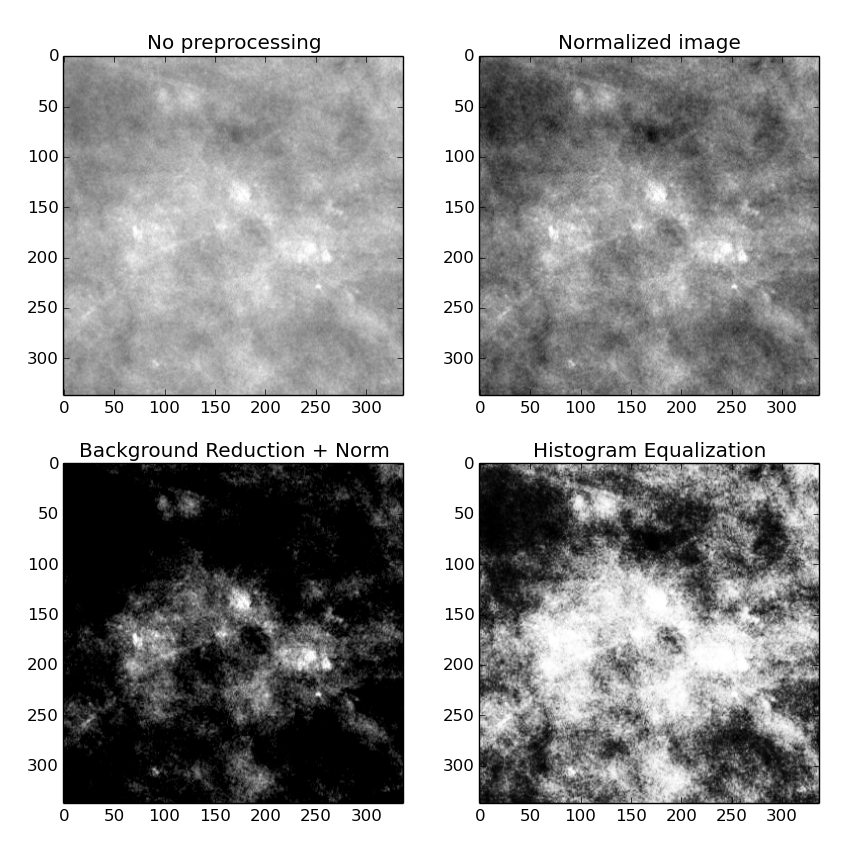
\includegraphics [width = 0.7\textwidth]{plots/mcDiffPreprocessings.png}
	\caption[Example of constrast adjustment techniques]{Example of simple contrast adjustment techniques applied to an image with a cluster of microcalcifications. Normalization takes the range of gray values and stretchs it up to linearly cover the entire range available. Background reduction assigns 0 to every pixel below the mean of the pixel values and applies normalization. Histogram equalization distributes the gray values more evenly in the histogram of the picture.}
	\label{fig:PreprocessingTechniques}
\end{figure}

We use background reduction plus normalization because it increases the signal to noise ratio, i.e., highlights lesions over normal breast tissue. On the downside, it also highlights dense structures (which could increase false positives) and may destroy important texture information by blending it with the background; using normalization only could produce better results. Unpreprocessed images seem too noisy and histogram equalization is too destructive for our purposes.

\paragraph{Data augmentation}
We augment each enhanced image by using 4 rotations (at 0°, 90°, 180° and 270°) of both the original image and a horizontally flipped version of it, thus we increase our data set by a factor of 8. Both rotations and reflections preserve the original label. In principle it is not neccesary to store the augmented images because they can be easily generated during training but if the disk space is not prohibitive explicitly storing them simplifies training.
%Does it affect to present all different augmentations of the same image in one batch rather than in different batches?

%TODO: Is feature normalization needed? It does put everything on -1 to 1 range (instead of 0-256, 0-2048, etc.). if it doesn't affect the results better do it

\paragraph{Resizing}
We have to resize the images to achieve the desired patch size. There is a couple of decisions to take in this part: the type of interpolation to use and whether image enhancement should be performed before or after resizing. After some experiments neither decisions proved to be very important for the resulting image patches. We choose the Lanczos interpolation recommended for downsizing in the PILLOW Python Image Library. Enhancements are executed on each particular patch before being scaled to their final size. Figure~\ref{fig:ResizingInterps} shows the effect of using the Bicubic or Lanczos interpolation scheme for resizing both before and after enhancement. Results are similar under all configurations.

\begin{figure}
	\centering
	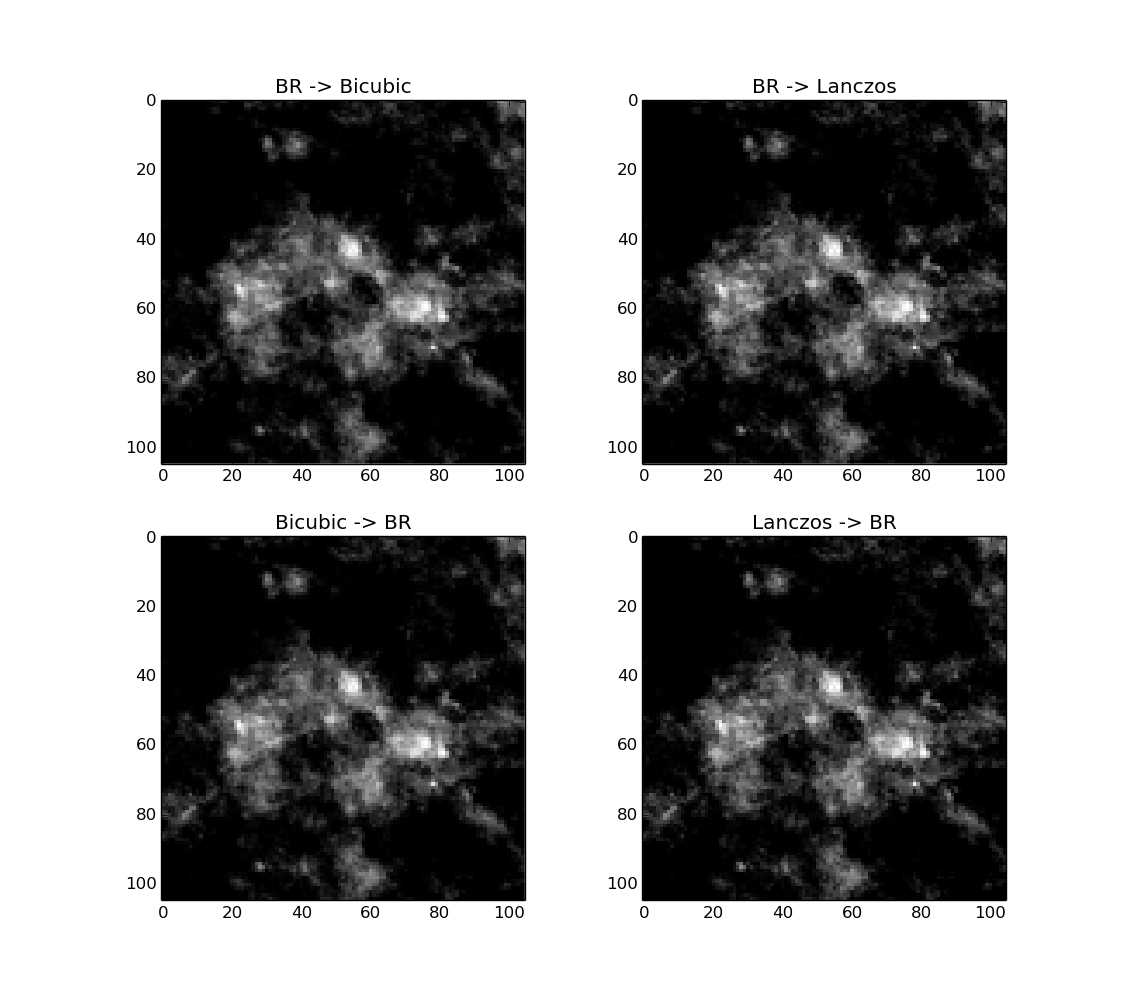
\includegraphics [width = 0.8\textwidth]{plots/mcDiffResizings.png}
	\caption[Example of resizing schemes]{Example of different resizing schemes applied to an image with a cluster of microcalcifications. Bicubic and Lanczos inteprolation is used for resizing an original 317 pixel image to 105 pixels before and after enhancement (background reduction plus normalization) as shown by the arrows in the subtitles. Results are virtually undistinguishable.}
	\label{fig:ResizingInterps}
\end{figure}

\paragraph{Storage}
For each mammogram we will generate a single 3-dimensional matrix ($64 \times 64 \times x$)  containing all $x$ preprocessed patches obtained from the mammogram. This matrix will be stored as a .pch file with the same name and on the same directory as the original image.


\section{Training}
	%Details about the practical decsiions taken to archotectures, and hyperparamters per experiments.

	\subsection{Data set}
	Yet to write
%	We have x number of images with x positives and negatives. Resunmied in Table...

	\subsection{Hardware}
	Training deep neural networks is computationally intensive and requires equipment with powerful GPUs. We enlist here the resources available for this thesis.
	\begin{table}[h]
		\centering
		\begin{tabular}{cp{3.9cm}p{1.7cm}p{1.8cm}cc}
		\hline
		\textbf{PC}	& \textbf{GPU}	& \textbf{HD}	& \textbf{CPU}	& \textbf{RAM}	& \textbf{\#} \\
		\hline
		Personal	& Nvidia NVS 5400M \newline 96 cores, 1GB, 2.1 compatibility, 29 GB/s	& 57 GB \newline (36 free)	& i5-3210M \newline 2.5GHz	& 4 GB	& 1 \\
		A4-401	& Nvidia Quadro K620 \newline 384 cores, 2GB, 5.0 compatibility, 29 GB/s & 240 GB \newline (230 free)	& i5-4570 \newline 3.2GHz	& 8 GB	& 27\\

		\hline
		\end{tabular}
		\caption{Available hardware for experiments}
	\end{table}
	% We did our experiments in x computers from A3-401

	\subsection{Architecture}
	Using the advice in Section~\ref{subsec:PracticalDL} we decided to use a simple network with six convolutional layers and two fully connected layers with the following architecture:
	\begin{table}[h]
		\centering
		\begin{tabular}{lccccr}
		\hline
		\textbf{Layer} & \textbf{Filter} & \textbf{Stride} &\textbf{Pad} & \textbf{Volume} & \textbf{Params} \\
		\hline
		\texttt{INPUT}	& -	& - & - & $127 \times 127 \times 1$ & -\\
		\texttt{CONV -> RELU} & $5 \times 5$ & 2 & 2 & $64 \times 64 \times 64$ & 1\,625\\
		\texttt{CONV -> RELU} & $3 \times 3$ & 1 & 1 & $64 \times 64 \times 64$ & 36\,928\\
		\texttt{MAXPOOL} & $2 \times 2$ & 2 & 0 & $32 \times 32 \times 64$ & -\\
		\texttt{CONV -> RELU} & $3 \times 3$ & 1 & 1 & $32 \times 32 \times 96$ & 55\,392\\
		\texttt{CONV -> RELU} & $3 \times 3$ & 1 & 1 & $32 \times 32 \times 96$ & 83\,040\\
		\texttt{MAXPOOL} & $2 \times 2$ & 2 & 0 & $16 \times 16 \times 96$ & -\\
		\texttt{CONV -> RELU} & $3 \times 3$ & 1 & 1 & $16 \times 16 \times 128$ & 110\,720\\
		\texttt{CONV -> RELU} & $3 \times 3$ & 1 & 1 & $16 \times 16 \times 128$ & 147\,584\\
		\texttt{MAXPOOL} & $2 \times 2$ & 2 & 0 & $8 \times 8 \times 128$ & -\\
		\texttt{FC -> RELU} & $8 \times 8$ & - & - & $1 \times 1 \times 512$ & 4\,194\,816\\
		\texttt{FC -> SIGMOID} & $1 \times 1$ & - & - & $1 \times 1 \times 1$ & 513 \\
		\hline
		\end{tabular}
		\label{tab:convNetArchitecture}
		\caption[Selected Convolutional Network Architecture]{Architecture of the network used for experiments. It shows the filter, stride and padding used in each layer as well as the resulting volume and the number of learnable parameters per layer.}
	\end{table}

	The first convolutional layer uses a $5 \times 5$ filter with stride 2 (padding 2) to reduce the input spatial size from $127 \times 127$ to $64 \times 64$. After that all filters are $3 \times 3$ with stride 1 (padding 1), which preserves the spatial size and the pooling is $2\times 2$ stride 2 (padding 0) which reduces the spatial size by a half. This architecture has 4.63 million learnable parameters. 

	In case the input was size $64 \times 64$ pixels we could replace use a $3 \times 3$ filter with stride 1 in the first convolutional layer and leave everything else unchanged. For an all convolutional architecture we could replace all pooling layers by a $5 \times 5$ filter  with stride 2 and use input images of size of $113 \times 113$ or $129 \times 129$.

	\subsection{Evaluation}
	When dividing the data set we make sure \textit{all} image patches obtained from the same patient are assigned to either the training set or test set (not distributed) to avoid any possible overfit to the test set. Given that our data is unbalanced, with far more negative than positive examples, we use PRAUC (see Section~\ref{subsec:Classification}) to choose between models for hyperparameter selection and as an overall performance metric. Other metrics are also reported for completeness. 

	We could also evaluate the network on all augmentations of an image and output the average prediction; in theory, this would give us better results. For simplicity, we do not apply it for model selection.

	For detection of lesions on entire mammograms we slide the trained convolutional network across the mammogram computing a per-pixel prediction. The generated heatmap preserves the size of the original mammogram (with some zero-padding) and can be presented side to side to the original mammogram as a CAD system. In case this heatmap is noisy (predictions changes abruptly from pixel to pixel) we could use a median or gaussian filter to smooth it out.% We do not evaluate the network on the entire mammogram (or per patient), we limit ourselves to show the results.

	\subsection{Software}
	We use Caffe~\cite{Jia2014} to train the networks and Python to develop any other tools (image retrieval and augmentation, model evaluation, figure generation, etc.).


\section{Implementation}

\section{Implementation details}
What library I used

\section{Evaluation metrics}
